\documentclass[11pt, oneside]{article}
\usepackage[margin=.9in]{geometry}
\usepackage{pgfplots}
\pgfplotsset{compat=default}
\newcommand{\cuckoo}{{\rm cuckoo}}
\newcommand{\hash}{{\rm siphash}}
\usepackage{hyperref}
\usepackage{listings}
\title{Cuckoo Cycle: \protect\\ a graph-theoretic proof-of-work system}
\author{John Tromp}
\begin{document}
\maketitle

\begin{abstract}
We introduce the first graph-theoretic proof-of-work system,
based on finding cycles in large random graphs.
Such problems are arbitrarily scalable and trivially verifiable.
Our implementation uses 1 bit per edge, and up to 1 bit per node.
We hypothesize that using significantly less causes superlinear slowdown.
\end{abstract}

\section{Introduction}
A ``proof of work'' (PoW) system allows a verifier to check with negligible
effort that a prover has expended a large amount of computational effort.
Originally introduced as a spam fighting measure, 
where the effort is the price paid by an email sender for demanding the
recipient's attention, they now form one of the cornerstones of
crypto-currencies.

As proof-of-work for new blocks of transactions,
Bitcoin~\cite{nakamoto2009bitcoin} adopted Adam Back's hashcash~\cite{back2002} proof-of-work.
This requires finding a nonce value such that
application of a cryptographic hash function (twofold SHA256 in Bitcoin's case)
to this nonce (and the rest of the block header) results in a number with
many leading 0s. The number of leading 0s is dynamically adjusted by the protocol
so as to maintain a certain average block interval (10-minutes for Bitcoin).

Since Bitcoin, many other crypto-currencies have adopted hashcash, with various
choices of underlying hash function. the most well-known being {\em scrypt} as
used in Litecoin.

Primecoin~\cite{king2013} introduced the notion of a number-theoretic proof-of-work,
as the first alternative to hashcash among crypto-currencies.
This requires finding long chains of nearly doubled prime numbers, with a certain
relation to the block header.
Current algorithms use a two-step process of filtering candidates by {\em sieving},
and applying pseudo-primality tests to remaining candidates.
These algorithms are somewhat complex and involve many trade-offs.
Recently, another prime-number based crypto-currency, Riecoin, was introduced, based
on finding clusters rather than chains of prime numbers.

\section{Graph-theoretic proofs-of-work}
We propose to base proofs-of-work on finding certain subgraphs in large pseudo-random graphs.
In the Erd\H{o}s-R\'{e}nyi model, denoted $G(N,M)$, a graph is chosen uniformly at random
from the collection of all graphs with $N$ nodes and $M$ edges. Instead, we choose edges
deterministically from the output of a keyed hash function, whose key could be chosen
uniformly at random. For a well-behaved hash function, these two classes of random graphs
should have nearly identical  properties.
Formally, fix a keyed hash function
$h: \{0,1\}^K \times \{0,1\}^W_i \rightarrow \{0,1\}^W_o$\footnote{hash functions generally
have arbitrary length inputs, but here we fix the input width at $W_i$ bits.},
and a small graph $H$ as a target subgraph.
Now pick a large number $N \leq 2^W_o$ as the number of nodes,
and $M \leq 2^{W_i-1}$ as the number of edges.
Each key $k \in \{0,1\}^K$ generates a graph $G_k = (V,E)$ where $V=\{v_0,\ldots,v_{N-1}\}$, and
\begin{equation}
E=\{(v_{h(k,2i) \bmod N},v_{h(k,2i+1) \bmod N}) | i \in [0,\ldots,M-1]\}
\end{equation}
The inputs $i \in [0,\ldots,M-1]$ are also called {\em nonces}.
The graph has a {\em solution} if $H$ occurs as a subgraph.
Denote the number of edges in h as $|H|$.
A proof of solution is an ordered list of $|H|$ nonces that generate the edges
of $H$'s occurrence in $G$.
Such a proof is verifiable in constant time, independent of $N$ and $M$.

A simple variation generates random bipartite graphs:
$G_k = (U \cup V,E)$ where $U=\{u_0,\ldots,u_{\frac{N}{2}-1}\}$, $V=\{v_0,\ldots,v_{\frac{N}{2}-1}\}$,
and
\begin{equation}
E=\{(u_{h(k,2i) \bmod \frac{N}{2}}, v_{h(k,2i+1) \bmod \frac{N}{2}}) | i \in [0,\ldots,M-1]\}
\end{equation}


The expected number of occurrences of $H$ as a subgraph of $G$ is a function of both $N$ and $M$,
and in many cases it is roughly a function of the ratio $\frac{M}{N}$.
For fixed $N$, the function is monotonically increasing in $M$.
To make the proof-of-work challenging, one chooses a value of $M$ that yields less than one
expected solution (but not much less).

\section{Cuckoo Cycle}
The simplest possible choice of subgraph is a fully connected one, or a {\em clique}.
While an interesting choice, akin to the number-theoretic notion of a prime-cluster,
as used in Riecoin, we leave its consideration to a future paper.
In this paper we focus on what is perhaps the next-simplest possible choice, the {\em cycle}.
Specifically, we propose the hash function \hash with a $K=128$ bit key, $W_i = W_O = 64$ input
and output bits, $N<2^{64}$ a 2-power, $M=N/2$, and $H$ a 42-cycle (more on that in a later section).
The reason for calling the resulting proof-of-work Cuckoo Cycle is that
inserting numbers in a Cuckoo hashtable naturally leads to forming cycles
in random bipartite graphs!

\section{Cuckoo hashing}
Introduced by Rasmus Pagh and Flemming Friche
Rodler~\cite{Pagh04cuckoohashing}, a cuckoo hashtable consists of two
same-sized tables each with its own hash function mapping a key to a table
location, providing two possible locations for each key.
Upon insertion of a new key, if both locations are already occupied by keys,
then one is kicked out and inserted in its alternate location, possibly
displacing yet another key, repeating the process until either a vacant
location is found, or some maximum number of iterations is reached.
The latter is bound to happen once cycles have formed in the {\em Cuckoo graph}.
This is a bipartite graph with a node for each location and an
edge for every key, connecting the two locations it can reside at.
It also matches the bipartite graph defined above if the cuckoo hashtable
were based on function $h$.
In fact, the insertion procedure suggests a simple algorithm for detecting cycles.

\section{Cycle detection in Cuckoo hashing}
We enumerate the $M$ nonces, but instead of storing the nonce itself as a key
in the Cuckoo hashtable, we store the alternate key location at the key
location, and forget about the nonce.  We thus maintain the {\em directed}
cuckoo graph, in which the edge for a key is directed from the location where
it resides to its alternate location.  Moving a key to its alternate location
thus corresponds to reversing its edge.  The outdegree of every node in this
graph is either 0 or 1.  When there are no cycles yet, the graph is a {\em
forest}, a disjoint union of trees.  In each tree, all edges are directed,
directly, or indirectly, to its {\em root}, the only node in the tree with
outdegree 0.  Initially there are just $N$ singleton trees consisting of
individual nodes which are all roots.
Addition of a new key causes a cycle if and only if its two endpoints are
nodes in the same tree, which we can test by following the path from each
endpoint to its root.
In case of different roots, we reverse all edges on the shorter of the two
paths, and finally create the edge for the new key itself, thereby joining
the two trees into one.
The left diagram below shows the directed cuckoo graph for header `39' on
$N=8+8$ nodes after adding edges
$(1,15),(2,12),(4,10),(2,15),(6,13),(5,10)$ and $(2,14)$ (nodes
with no incident edges are omitted for clarity).
In order to add the 8th edge $(5,13)$, we follow the paths $5 \rightarrow 10
\rightarrow 4$ and $13 \rightarrow 6$ to find different roots $4$ and $6$.
Since the latter path is shorter, we reverse it to $6 \rightarrow 13$ so we
can add the new edge as $(13 \rightarrow 5)$, resulting in the middle diagram.
In order to add to 9th edge
$(5,14)$ we now find the path from $5$ to be the shorter one, so we reverse
that and add the new edge as $(5 \rightarrow 14)$, resulting in the right diagram.
\begin{center}
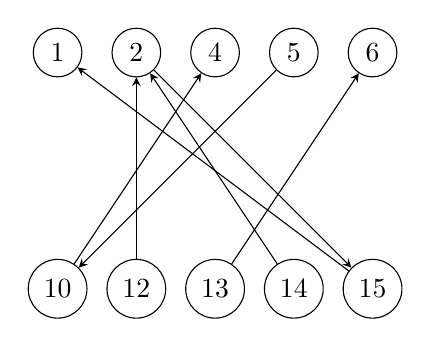
\begin{tikzpicture}[>=stealth]
\node  (1) at (1, 2) [shape=circle,draw] {1};
\node  (2) at (2, 2) [shape=circle,draw] {2};
\node  (4) at (3, 2) [shape=circle,draw] {4};
\node  (5) at (4, 2) [shape=circle,draw] {5};
\node  (6) at (5, 2) [shape=circle,draw] {6};
\node (10) at (1,-1) [shape=circle,draw] {10};
\node (12) at (2,-1) [shape=circle,draw] {12};
\node (13) at (3,-1) [shape=circle,draw] {13};
\node (14) at (4,-1) [shape=circle,draw] {14};
\node (15) at (5,-1) [shape=circle,draw] {15};
\draw [->] (15) -- (1);
\draw [->] (12) -- (2);
\draw [->] (10) -- (4);
\draw [->]  (2) -- (15);
\draw [->] (13) -- (6);
\draw [->]  (5) -- (10);
\draw [->] (14) -- (2);
\end{tikzpicture}\hspace{1cm}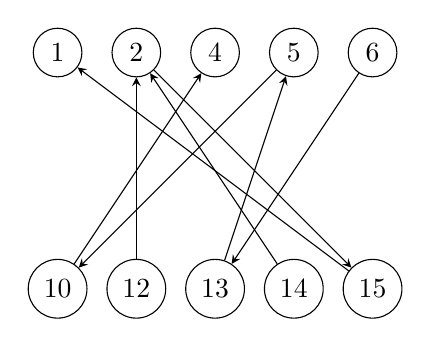
\begin{tikzpicture}[>=stealth]
\node  (1) at (1, 2) [shape=circle,draw] {1};
\node  (2) at (2, 2) [shape=circle,draw] {2};
\node  (4) at (3, 2) [shape=circle,draw] {4};
\node  (5) at (4, 2) [shape=circle,draw] {5};
\node  (6) at (5, 2) [shape=circle,draw] {6};
\node (10) at (1,-1) [shape=circle,draw] {10};
\node (12) at (2,-1) [shape=circle,draw] {12};
\node (13) at (3,-1) [shape=circle,draw] {13};
\node (14) at (4,-1) [shape=circle,draw] {14};
\node (15) at (5,-1) [shape=circle,draw] {15};
\draw [->] (15) -- (1);
\draw [->] (12) -- (2);
\draw [->] (10) -- (4);
\draw [->]  (2) -- (15);
\draw [->]  (6) -- (13);
\draw [->]  (5) -- (10);
\draw [->] (14) -- (2);
\draw [->] (13) -- (5);
\end{tikzpicture}\hspace{1cm}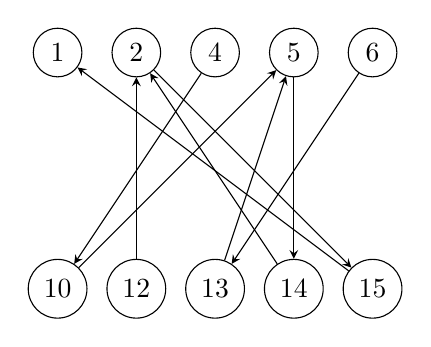
\begin{tikzpicture}[>=stealth]
\node  (1) at (1, 2) [shape=circle,draw] {1};
\node  (2) at (2, 2) [shape=circle,draw] {2};
\node  (4) at (3, 2) [shape=circle,draw] {4};
\node  (5) at (4, 2) [shape=circle,draw] {5};
\node  (6) at (5, 2) [shape=circle,draw] {6};
\node (10) at (1,-1) [shape=circle,draw] {10};
\node (12) at (2,-1) [shape=circle,draw] {12};
\node (13) at (3,-1) [shape=circle,draw] {13};
\node (14) at (4,-1) [shape=circle,draw] {14};
\node (15) at (5,-1) [shape=circle,draw] {15};
\draw [->] (15) -- (1);
\draw [->] (12) -- (2);
\draw [->]  (4) -- (10);
\draw [->]  (2) -- (15);
\draw [->]  (6) -- (13);
\draw [->] (10) -- (5);
\draw [->] (14) -- (2);
\draw [->] (13) -- (5);
\draw [->]  (5) -- (14);
\end{tikzpicture}
\end{center}
When adding the 10th edge $(4,12)$, we find the paths $4 \rightarrow 10
\rightarrow 5 \rightarrow 14 \rightarrow 2 \rightarrow 15 \rightarrow 1$ and
$12 \rightarrow 2 \rightarrow 15 \rightarrow  1$ with equal roots.
In this case, we can compute the length of the resulting cycle as
1 plus the sum of the path-lengths to the node where the two paths first join.
In the diagram, the paths first join at $2$, and the cycle length is computed as $1+4+1=6$.

\section{Union-find}
The above representation of the directed cuckoo graph is an example of
a {\em disjoint-set data structure}~\cite{wikidsds2014}, and our algorithm is
closely related to the well-known union-find algorithm, where the find operation
determines which subset an element is in, and the union operation joins two subsets
into a single one. For each edge addition to the cuckoo graph we perform the equivalent
of two find operations and one union operation.
The difference is that the union-find algorithm is free to add
directed edges between arbitrary elements. Thus it can join two subsets by adding an edge
from one root to another, with no need to reverse any edges. Conversely, our algorithm
can be seen as the first one that solves the union-find problem by maintaining
a direction on all union operations while keeping the maximum outdegree at 1.

\section{Cuckoo Cycle basic algorithm}
The above algorithm for inserting edges and detecting cycles forms the basis
for our basic proof-of-work algorithm.
If a cycle of length $L$ is found, then we solved the problem, and recover the proof
by storing the cycle edges in a set and enumerating nonces once more to see which ones
generate edges in the set.
If a cycle of a different length is found, then we keep the graph acyclic by ignoring the edge.
There is some probability of overlooking other $L$-cycles
through that edge, but in the important case of having few cycles
in the cuckoo graph to begin with, it hardly affects the rate of solution finding.

This algorithm is available online at \url{https://github.com/tromp/cuckoo}
as either the C-program simple\_miner.cpp or the Java program SimpleMiner.java.
A proof verifier is available as cuckoo.c or Cuckoo.java, while the repository
also has a Makefile, as well as the latest version of this paper.
% `make test' tests everything.
`make example' reproduces the example shown above.
The simple program uses 32 bits per node to represent the directed cuckoo graph,
plus about 64KB per thread for 2 auxiliary arrays.
The left plot below shows both the total runtime in seconds and the runtime of just
the hash computation, as a function of (log)size. The latter is purely
linear, while the former is superlinear due to increasing memory latency
as the nodes no longer fit in cache. The right plot show this more clearly
as the percentage of hashing to total runtime, ending up around 5\%.

\begin{center}
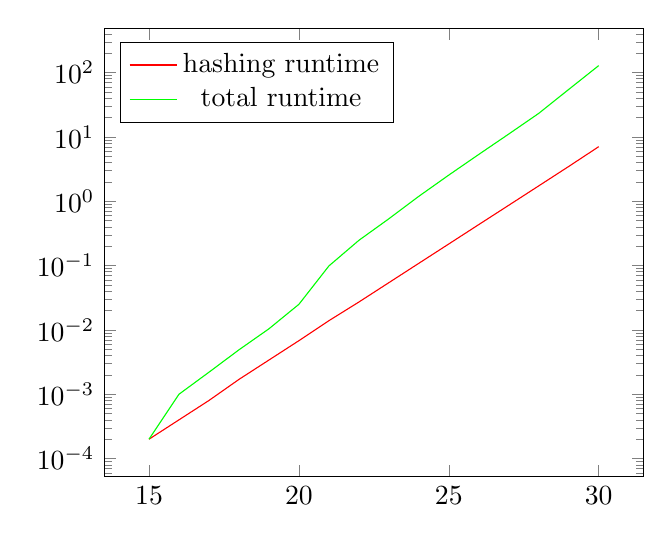
\begin{tikzpicture}
\begin{axis}[ymode=log, legend pos=north west]
\addplot[color=red] coordinates {
% (10,0.0000) (11,0.0000) (12,0.0000) (13,0.0001) (14,0.0001)
(15,0.0002) (16,0.0004) (17,0.0008) (18,0.0017) (19,0.0034)
(20,0.0068) (21,0.0139) (22,0.0271) (23,0.0542) (24,0.1084)
(25,0.2166) (26,0.4336) (27,0.8658) (28,1.7322) (29,3.4719)
(30,7.0389) };
\addlegendentry{hashing runtime}
\addplot[color=green] coordinates {
% (10,0.0000) (11,0.0000) (12,0.0001) (13,0.0001) (14,0.0003)
(15,0.0002) (16,0.0010) (17,0.0022) (18,0.0049) (19,0.0104)
(20,0.0250) (21,0.0986) (22,0.2465) (23,0.5332) (24,1.1922)
(25,2.5505) (26,5.3394) (27,11.0793) (28,23.1984) (29,54.6811)
(30,128.1682) };
\addlegendentry{total runtime}
\end{axis}
\end{tikzpicture}
\hspace{1cm}
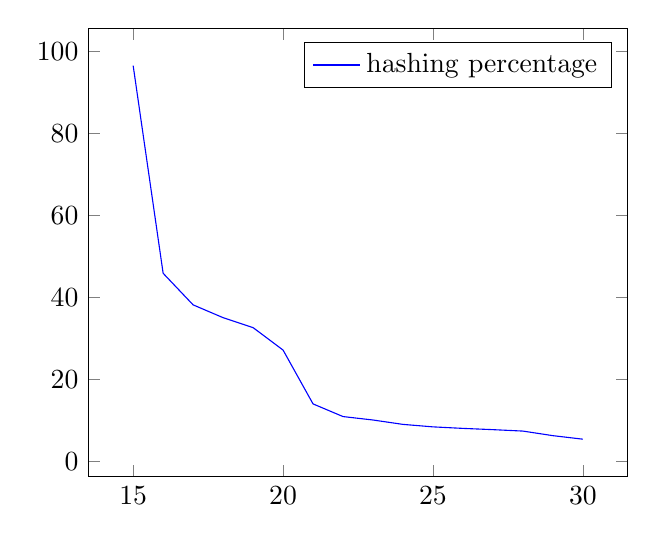
\begin{tikzpicture}
\begin{axis}[legend pos=north east]
\addplot[color=blue] coordinates {
% (10,38.8889) (11,33.3333) (12,45.1613) (13,39.8496) (14,44.6154)
(15,96.5217) (16,45.9119) (17,38.2180) (18,35.0988) (19,32.6724)
(20,27.2076) (21,14.0874) (22,11.0014) (23,10.1635) (24,9.0964)
(25,8.4921) (26,8.1215) (27,7.8144) (28,7.4670) (29,6.3494)
(30,5.4919) };
\addlegendentry{hashing percentage}
\end{axis}
\end{tikzpicture}
\end{center}

The left plot below shows the probability of finding a 42-cycle as a function
of the percentage edges/nodes (relative easiness), while the right plot shows the average number of
memory reads and writes per edge as a function of the percentage
nonce/easiness (progress through main loop). Both were determined from 10000 runs at size $2^{20}$;
results at size $2^{25}$ look almost identical.
In total the program averages 3.3 reads and 1.1 writes per edge.

\begin{center}
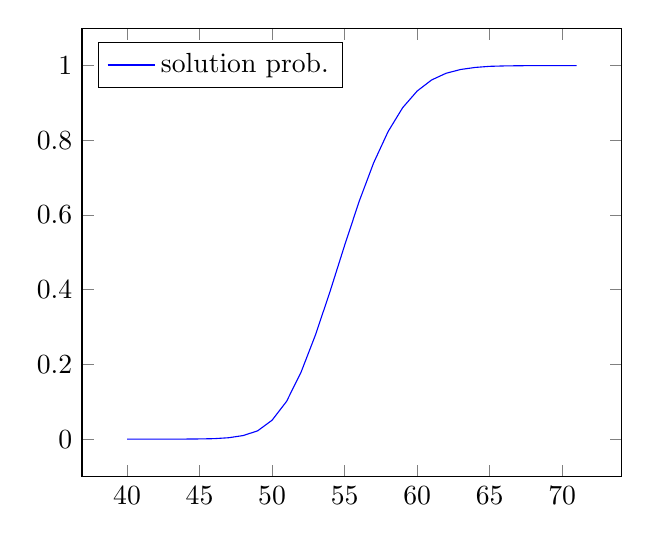
\begin{tikzpicture}
\begin{axis}[legend pos=north west]
\addplot[color=blue] coordinates {
(40,0) (41,0.00001) (42,0.00003) (43,0.0001) (44,0.00031) (45,0.00067)
(46,0.00141) (47,0.00385) (48,0.00967) (49,0.02222) (50,0.05076)
(51,0.10117) (52,0.17953) (53,0.27993) (54,0.39581) (55,0.51873)
(56,0.63614) (57,0.73955) (58,0.82352) (59,0.88719) (60,0.93182)
(61,0.9616) (62,0.97949) (63,0.98956) (64,0.99503) (65,0.99799)
(66,0.99907) (67,0.9996) (68,0.99989) (69,0.99997) (70,0.99998) (71,1) };
\addlegendentry{solution prob.}
\end{axis}
\end{tikzpicture}
\hspace{1cm}
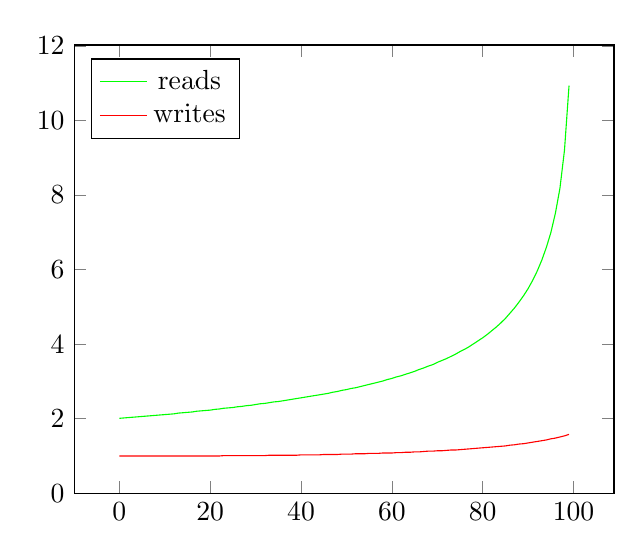
\begin{tikzpicture}
\begin{axis}[ymin=0, legend pos=north west]
\addplot[color=green] coordinates {
(0,2.01) (1,2.02) (2,2.03) (3,2.04) (4,2.05) (5,2.06) (6,2.07) (7,2.08) (8,2.09) (9,2.10) (10,2.11) (11,2.12) (12,2.13) (13,2.15) (14,2.16) (15,2.17) (16,2.18) (17,2.20) (18,2.21) (19,2.22) (20,2.23) (21,2.25) (22,2.26) (23,2.28) (24,2.29) (25,2.30) (26,2.32) (27,2.33) (28,2.35) (29,2.36) (30,2.38) (31,2.40) (32,2.41) (33,2.43) (34,2.45) (35,2.46) (36,2.48) (37,2.50) (38,2.52) (39,2.54) (40,2.56) (41,2.58) (42,2.60) (43,2.62) (44,2.64) (45,2.66) (46,2.68) (47,2.71) (48,2.73) (49,2.76) (50,2.78) (51,2.81) (52,2.83) (53,2.86) (54,2.89) (55,2.92) (56,2.95) (57,2.98) (58,3.01) (59,3.05) (60,3.08) (61,3.12) (62,3.15) (63,3.19) (64,3.23) (65,3.27) (66,3.32) (67,3.36) (68,3.41) (69,3.45) (70,3.51) (71,3.56) (72,3.61) (73,3.67) (74,3.73) (75,3.80) (76,3.86) (77,3.93) (78,4.01) (79,4.09) (80,4.17) (81,4.26) (82,4.36) (83,4.46) (84,4.57) (85,4.69) (86,4.83) (87,4.97) (88,5.13) (89,5.30) (90,5.49) (91,5.71) (92,5.96) (93,6.25) (94,6.59) (95,6.99) (96,7.51) (97,8.18) (98,9.20) (99,10.93) };
\addlegendentry{reads}
\addplot[color=red] coordinates {
(0,1.00) (1,1.00) (2,1.00) (3,1.00) (4,1.00) (5,1.00) (6,1.00) (7,1.00) (8,1.00) (9,1.00) (10,1.00) (11,1.00) (12,1.00) (13,1.00) (14,1.00) (15,1.00) (16,1.00) (17,1.00) (18,1.00) (19,1.00) (20,1.00) (21,1.00) (22,1.00) (23,1.01) (24,1.01) (25,1.01) (26,1.01) (27,1.01) (28,1.01) (29,1.01) (30,1.01) (31,1.01) (32,1.01) (33,1.02) (34,1.02) (35,1.02) (36,1.02) (37,1.02) (38,1.02) (39,1.02) (40,1.03) (41,1.03) (42,1.03) (43,1.03) (44,1.03) (45,1.04) (46,1.04) (47,1.04) (48,1.04) (49,1.05) (50,1.05) (51,1.05) (52,1.06) (53,1.06) (54,1.06) (55,1.07) (56,1.07) (57,1.07) (58,1.08) (59,1.08) (60,1.08) (61,1.09) (62,1.09) (63,1.10) (64,1.10) (65,1.11) (66,1.11) (67,1.12) (68,1.13) (69,1.13) (70,1.14) (71,1.14) (72,1.15) (73,1.16) (74,1.16) (75,1.17) (76,1.18) (77,1.19) (78,1.20) (79,1.21) (80,1.22) (81,1.23) (82,1.24) (83,1.25) (84,1.26) (85,1.27) (86,1.29) (87,1.30) (88,1.32) (89,1.33) (90,1.35) (91,1.37) (92,1.39) (93,1.41) (94,1.43) (95,1.46) (96,1.48) (97,1.51) (98,1.54) (99,1.58) };
\addlegendentry{writes}
\end{axis}
\end{tikzpicture}
\end{center}

\section{Difficulty control}
Relative easiness (the ratio $E/N$) determines a base level of difficulty,
which may suffice for applications where difficulty is to remain fixed.
The ratio $E/N=1$ is suitable when a practically guaranteed solution is desired,
For crypto currencies, where difficulty must scale in precisely
controlled manner across a huge range, adjusting easiness is not suitable.
The implementation default $E/N=1/2$ gives a solution probability of roughly $2.2\%$,
while the average number of cycles found increases slowly with size; from 2 at $2^{20}$
to 3 at $2^{30}$.
For further control, a difficulty target $0 < T < 2^{256}$ is introduced,
and we impose the additional constraint that the sha256 digest of the
cycle nonces in ascending order be less than $T$, thus
reducing the success probability by a factor $2^{256}/T$.

\section{Edge Trimming}
Dave Andersen~\cite{dga2014} suggested drastically reducing the number of edges
our basic algorithm has to process, by repeatedly identifying nodes of degree one
and eliminating its incident edge. Such {\em leaf edges} can never be part of a cycle.
This works whenever the number of edges $M$, is at most half the number of nodes $N$,
since the expected degree of a node is then at most 1.

This is implemented in our main algorithm in cuckoo\_miner.h
It maintains a set of {\em alive} edges as a bit vector. Initially all edges are alive.
In each of a given number of trimming rounds, it shrinks this set as follows.
A vector of 2-bit degree counters, one per u-node, is initialized to all zeroes.
Next, for all alive edges, compute its u-endpoint and increase the corresponding counter,
capping the value at 2.
Next, for all alive edges, compute its u-endpoint and if the corresponding counter is less than 2,
set the edge to be not-alive.
These steps are repeated for the other partition, of v-nodes.
Preprocessor symbol PART\_BITS, whose value we'll denote as $B$,
allows for trading-off node counter storage for time,
by processing the nodes in multiple passes depending on the value of their least significant bits.
The memory usage is $M$ bits for the alive set and $N / 2^{B}$ for the counters.

After all edge trimming rounds, the counter memory is freed, and allocated to a
custom cuckoo\_hashtable that presents the same interface as the simple array in
the basic algorithm, but gets by with much fewer locations, as long as its {\em load},
the ratio of remaining edges to number of locations, is significantly less than 1.

The number of trimming rounds, which can be set with option {\tt -n}, defaults to
$2^{1+(B+3)*(B+4)/2}$, which achieves a load close to $50\%$.

\section{Memory-hardness}
Reducing memory usage to a under 1 bit per edge is quite challenging.
One approach is to maintain the set of alive edges in three parts:
\begin{itemize}
\item one part that has a density less than one-half and can be compressed using
e.g. arithmetic coding.
\item one part that is stored uncompressed.
\item remaining edges are not stored and considered all alive.
\end{itemize}
Let's say we devote $A$ percent of $N/2$ bits (regular alive storage) to this, and another
$B$ percent to vertex degree counters. The left plot below shows how well a given fraction
of edges can be compressed (the entropy of live probability)
by repeatedly removing leaf edges within this fraction. Most
of this removal is achieved in 4 rounds of trimming, with each round of trimming requiring
$2\cdot2\cdot\lceil \frac{2\cdot 100}{B} \rceil$ passes over all alive edges
(one factor of 2 for $U \cup V$, another for writing and then reading degree counts).
(Re-)compressing the current stored fraction frees up some of $A$,
which allows us to transfer part of the unstored edges into a new uncompressed part.
Repeating this process will ultimately trim all but a small fraction of edges.
The plot on the right shows how many passes are needed as a function of the total
memory usage $A+B$ where the split between $A$ and $B$ is always chosen optimally.
Clearly this time-memory trade-off is highly nonlinear and impractical below 50\%.

\begin{center}
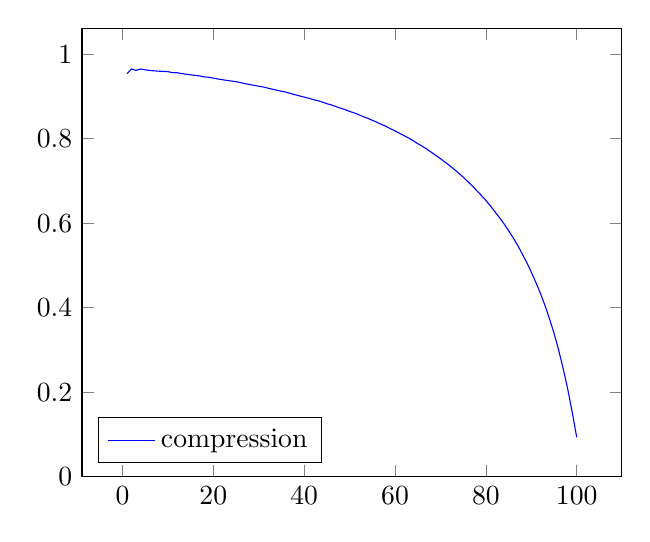
\begin{tikzpicture}
\begin{axis}[ymin=0, legend pos=south west]
\addplot [color=blue] coordinates {
( 1,0.9544) ( 2,0.9652) ( 3,0.9618) ( 4,0.9652) ( 5,0.9632)
( 6,0.9618) ( 7,0.9608) ( 8,0.9600) ( 9,0.9594) (10,0.9589)
(11,0.9565) (12,0.9563) (13,0.9544) (14,0.9528) (15,0.9513)
(16,0.9500) (17,0.9488) (18,0.9464) (19,0.9455) (20,0.9435)
(21,0.9415) (22,0.9398) (23,0.9381) (24,0.9366) (25,0.9352)
(26,0.9328) (27,0.9305) (28,0.9284) (29,0.9263) (30,0.9244)
(31,0.9226) (32,0.9199) (33,0.9173) (34,0.9149) (35,0.9125)
(36,0.9103) (37,0.9072) (38,0.9043) (39,0.9014) (40,0.8987)
(41,0.8960) (42,0.8926) (43,0.8902) (44,0.8869) (45,0.8830)
(46,0.8800) (47,0.8762) (48,0.8725) (49,0.8690) (50,0.8647)
(51,0.8613) (52,0.8571) (53,0.8523) (54,0.8484) (55,0.8437)
(56,0.8392) (57,0.8339) (58,0.8295) (59,0.8236) (60,0.8186)
(61,0.8129) (62,0.8073) (63,0.8017) (64,0.7954) (65,0.7884)
(66,0.7823) (67,0.7755) (68,0.7679) (69,0.7604) (70,0.7529)
(71,0.7447) (72,0.7366) (73,0.7277) (74,0.7189) (75,0.7093)
(76,0.6988) (77,0.6884) (78,0.6772) (79,0.6660) (80,0.6539)
(81,0.6410) (82,0.6271) (83,0.6132) (84,0.5984) (85,0.5825)
(86,0.5656) (87,0.5476) (88,0.5274) (89,0.5070) (90,0.4842)
(91,0.4600) (92,0.4342) (93,0.4056) (94,0.3739) (95,0.3399)
(96,0.3006) (97,0.2566) (98,0.2085) (99,0.1531) (100,0.0930)
};
\addlegendentry{compression}
\end{axis}
\end{tikzpicture}\hspace{1cm}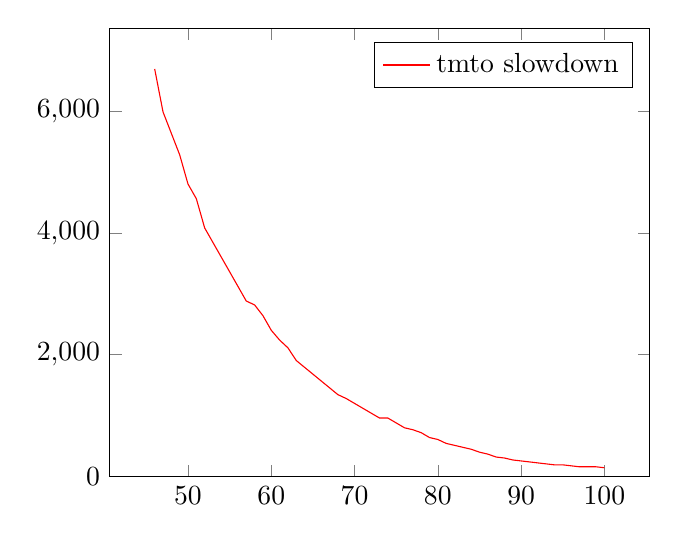
\begin{tikzpicture}
\begin{axis}[ymin=0, legend pos=north east]
\addplot [color=red] coordinates {
(46,6688) (47,5984) (48,5632) (49,5280) (50,4800)
(51,4560) (52,4080) (53,3840) (54,3600) (55,3360)
(56,3120) (57,2880) (58,2816) (59,2640) (60,2400)
(61,2240) (62,2112) (63,1904) (64,1792) (65,1680)
(66,1568) (67,1456) (68,1344) (69,1280) (70,1200)
(71,1120) (72,1040) (73,960) (74,960) (75,880)
(76,800) (77,768) (78,720) (79,640) (80,608)
(81,544) (82,512) (83,480) (84,448) (85,400)
(86,368) (87,320) (88,304) (89,272) (90,256)
(91,240) (92,224) (93,208) (94,192) (95,192)
(96,176) (97,160) (98,160) (99,160) (100,144)
};
\addlegendentry{tmto slowdown}
\end{axis}
\end{tikzpicture}
\end{center}

\section{Parallelization}
The implementation allows the number of threads to be set with option {\tt -t}.
For $0\leq t < T$, thread $t$ processes all nonces $t \bmod T$.
Parallelization in the basic algorithm presents some minor algorithmic challenges.
Paths from an edge's two endpoints
are not well-defined when other edge additions and path reversals are still in progress.
One example of such a path conflict is the check for duplicate edges yielding a false negative,
if in between checking the two endpoints, another thread reverses a path through those nodes.
Another is the inadvertent creation of cycles when a reversal in progress hampers another thread's
path following causing it to overlook root equality.
Thus, in a parallel implementation, path following can no longer be assumed to terminate.
Instead of using a cycle detection algorithm such as~\cite{1980-brent-cycles}, our implementation
notices when the path length exceeds MAXPATHLEN (8192 by default),
and reports whether this is due to a path conflict.

In the main algorithm, cycle detection only takes a small fraction of total runtime and
the conflicts above could be avoided altogether by running the cycle detection single threaded.
We therefore turn our attention to parallelization of edge trimming.

To be expanded...

\begin{center}
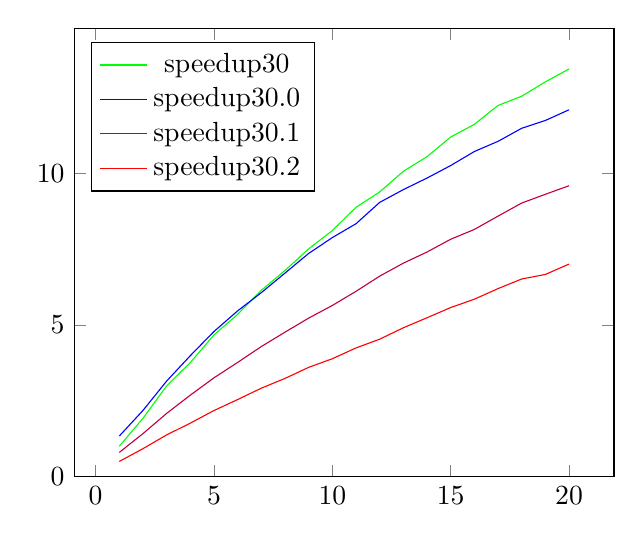
\begin{tikzpicture}
\begin{axis}[ymin=0, legend pos=north west]
\addplot [color=green] coordinates {
(1,1.000) (2,1.921) (3,2.988) (4,3.757) (5,4.668) 
(6,5.347) (7,6.138) (8,6.792) (9,7.504) (10,8.108) 
(11,8.873) (12,9.380) (13,10.061) (14,10.543) (15,11.190) 
(16,11.608) (17,12.231) (18,12.535) (19,13.008) (20,13.433) 
};
\addlegendentry{speedup30}
\addplot [color=blue] coordinates {
(1,1.336) (2,2.179) (3,3.148) (4,3.984) (5,4.781) 
(6,5.462) (7,6.061) (8,6.706) (9,7.354) (10,7.876) 
(11,8.333) (12,9.036) (13,9.457) (14,9.838) (15,10.250) 
(16,10.713) (17,11.048) (18,11.479) (19,11.736) (20,12.088) 
};
\addlegendentry{speedup30.0}
\addplot [color=purple] coordinates {
(1,0.795) (2,1.416) (3,2.082) (4,2.683) (5,3.255) 
(6,3.762) (7,4.285) (8,4.759) (9,5.222) (10,5.639) 
(11,6.105) (12,6.605) (13,7.033) (14,7.400) (15,7.821) 
(16,8.144) (17,8.583) (18,9.014) (19,9.303) (20,9.585) 
};
\addlegendentry{speedup30.1}
\addplot [color=red] coordinates {
(1,0.498) (2,0.919) (3,1.373) (4,1.761) (5,2.176) 
(6,2.538) (7,2.913) (8,3.234) (9,3.599) (10,3.883) 
(11,4.239) (12,4.527) (13,4.903) (14,5.234) (15,5.570) 
(16,5.845) (17,6.194) (18,6.511) (19,6.661) (20,7.003) 
};
\addlegendentry{speedup30.2}
\end{axis}
\end{tikzpicture}\hspace{1cm}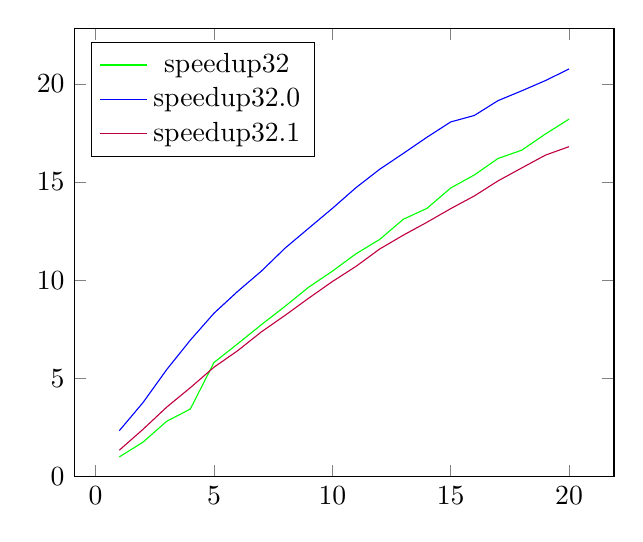
\begin{tikzpicture}
\begin{axis}[ymin=0, legend pos=north west]
\addplot [color=green] coordinates {
(1,1.000) (2,1.752) (3,2.813) (4,3.439) (5,5.810) 
(6,6.762) (7,7.732) (8,8.669) (9,9.646) (10,10.460) 
(11,11.348) (12,12.077) (13,13.107) (14,13.663) (15,14.698) 
(16,15.363) (17,16.202) (18,16.623) (19,17.446) (20,18.207) 
};
\addlegendentry{speedup32}
\addplot [color=blue] coordinates {
(1,2.337) (2,3.767) (3,5.445) (4,6.949) (5,8.319) 
(6,9.432) (7,10.462) (8,11.632) (9,12.648) (10,13.658) 
(11,14.717) (12,15.652) (13,16.461) (14,17.286) (15,18.063) 
(16,18.393) (17,19.149) (18,19.647) (19,20.169) (20,20.761) 
};
\addlegendentry{speedup32.0}
\addplot [color=purple] coordinates {
(1,1.343) (2,2.404) (3,3.534) (4,4.526) (5,5.570) 
(6,6.410) (7,7.367) (8,8.208) (9,9.085) (10,9.932) 
(11,10.707) (12,11.590) (13,12.297) (14,12.954) (15,13.647) 
(16,14.294) (17,15.060) (18,15.718) (19,16.371) (20,16.804) 
};
\addlegendentry{speedup32.1}

\end{axis}
\end{tikzpicture}
\end{center}

\section{Choice of cycle length}
Extremely small cycle lengths risk the feasibility of alternative algorithms with better performance.
For example, for $L=2$ the problem reduces to finding a birthday collision
as in the Momentum proof-of-work.
It is conceivable however that the Cuckoo representation is already optimal for $L=4$.
In order to keep proof size manageable, the cycle length should not be too large either.
We consider 20-64 to be a healthy range, which averages to 42.
The plot below shows the distribution of cycle lengths found for sizes $2^{10},2^{15},2^{20},2^{25}$,
as determined from 100000,100000,10000, and 10000 runs respectively. The tails of the distributions
beyond $L=100$ are not shown. For reference, the longest cycle found was of length 2120.

\begin{center}
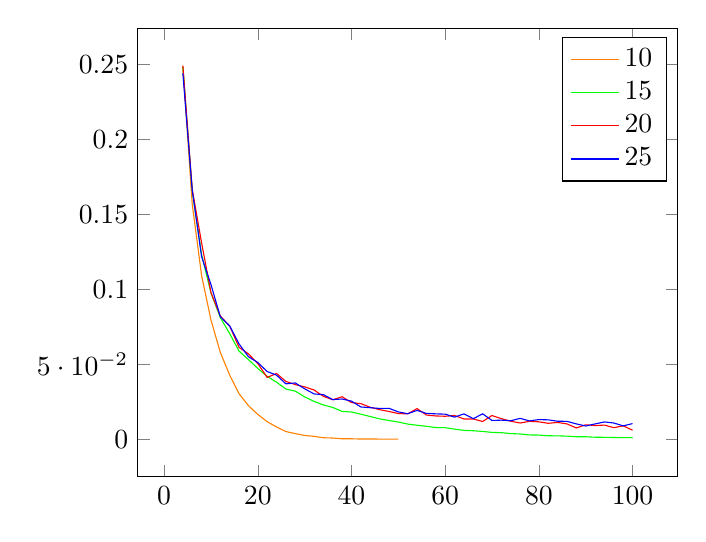
\begin{tikzpicture}
\begin{axis}
\addplot[color=orange] coordinates {
(4,0.24862) (6,0.15673) (8,0.10907) (10,0.07952) (12,0.05783) (14,0.04269) (16,0.0303)
(18,0.02237) (20,0.01653) (22,0.01168) (24,0.00815) (26,0.00511) (28,0.00374) (30,0.00251)
(32,0.00191) (34,0.00098) (36,0.00079) (38,0.00029) (40,0.0003) (42,0.00011) (44,0.00018)
(46,8e-05) (48,2e-05) (50,3e-05) };
\addlegendentry{10}
\addplot[color=green] coordinates {
(4,0.24822) (6,0.16551) (8,0.12317) (10,0.09749) (12,0.08105) (14,0.07036) (16,0.05871) (18,0.05308)
(20,0.04717) (22,0.04189) (24,0.03801) (26,0.03342) (28,0.03205) (30,0.02822) (32,0.02521)
(34,0.02282) (36,0.0212) (38,0.01852) (40,0.01814) (42,0.01668) (44,0.01511) (46,0.01356)
(48,0.01246) (50,0.01145) (52,0.0101) (54,0.0093) (56,0.00861) (58,0.00778) (60,0.00768)
(62,0.00672) (64,0.00589) (66,0.00565) (68,0.00517) (70,0.00455) (72,0.00435) (74,0.00375)
(76,0.00348) (78,0.00286) (80,0.00276) (82,0.0023) (84,0.00224) (86,0.00204) (88,0.00165)
(90,0.00164) (92,0.00134) (94,0.00126) (96,0.00114) (98,0.00103) (100,0.00101) };
\addlegendentry{15}
\addplot[color=red] coordinates {
(4,0.249) (6,0.1666) (8,0.1309) (10,0.0977) (12,0.0821) (14,0.0754) (16,0.0612) (18,0.0569)
(20,0.0504) (22,0.0412) (24,0.0438) (26,0.0385) (28,0.0364) (30,0.0349) (32,0.0328) (34,0.0286)
(36,0.0263) (38,0.0283) (40,0.0244) (42,0.0237) (44,0.0213) (46,0.0197) (48,0.0185) (50,0.0171)
(52,0.0169) (54,0.0204) (56,0.0161) (58,0.0155) (60,0.0153) (62,0.0158) (64,0.0135) (66,0.0135)
(68,0.0118) (70,0.0158) (72,0.0137) (74,0.012) (76,0.0108) (78,0.0119) (80,0.0116) (82,0.0106)
(84,0.0112) (86,0.0102) (88,0.0075) (90,0.0096) (92,0.0091) (94,0.0094) (96,0.0077) (98,0.0089)
(100,0.006) };
\addlegendentry{20}
\addplot[color=blue] coordinates {
(4,0.2439) (6,0.1661) (8,0.1216) (10,0.1031) (12,0.0816) (14,0.0755) (16,0.0635) (18,0.055) (20,0.0511) (22,0.0451) (24,0.0427) (26,0.0369) (28,0.0375) (30,0.0336) (32,0.0302) (34,0.0297) (36,0.0264) (38,0.0268) (40,0.0254) (42,0.0215) (44,0.021) (46,0.0205) (48,0.0206) (50,0.0182) (52,0.017) (54,0.0192) (56,0.0172) (58,0.0169) (60,0.0167) (62,0.0147) (64,0.0169) (66,0.0137) (68,0.0169) (70,0.0125) (72,0.0127) (74,0.0123) (76,0.0139) (78,0.0122) (80,0.0131) (82,0.0129) (84,0.012) (86,0.0119) (88,0.0102) (90,0.0088) (92,0.0102) (94,0.0115) (96,0.0108) (98,0.0089) (100,0.0104) };
\addlegendentry{25}
\end{axis}
\end{tikzpicture}
\end{center}

% \section{Choice of memory size}
% The memory requirement should exceed that of the largest available
% single-chip memory to enforce off-chip latencies.
% It should also be a
% significant fraction of the typical memory of a botnet computer,
% With a significant risk of sending machines into swap-hell and
% likely alerting its owner, botnet operators will refrain from deploying
% Cuckoo Cycle, preferring other proof-of-work schemes whose smaller memory
% footprint allows them to stay under the radar.
% With memory sizes doubling roughly every 18 months, 16GB will become
% commonplace in a few years.
The main implementation can easily handle $N=2^{43}$ nodes which uses 1TB of memory.

% \section{Memory latency; the great equalizer}
% While cpu-speed and (sequential) memory bandwidth are highly variable across
% time and architectures, main memory latencies have remained relatively
% stable. This suggests making the proof-of-work system latency-bound in order
% to level the mining playing field.
% We introduce the very first graph-theoretic proof-of-work system.
% which aims to satisfy most of the above properties,
% except for parallel-hardness (see the later section on parallelizability).
% Amazingly, it amounts to little more than enumerating nonces and storing them
% in a hashtable. While all hashtables break down when trying to store more
% items than it was designed to handle, in one hashtable design in particular
% this breakdown is of a special nature that can be turned into a concise and
% easily verified proof. Enter the cuckoo hashtable.

\section{Computation versus memory}
Starting out at 32 leading zeroes in 2009, Bitcoin difficulty
has steadily climbed and is currently
at 64, representing an incredible $2^{64}/10$ double-hashes per minute.
This growth was enabled by the migration of hash computation from 
desktop processors (CPUs) to graphics-card processors (GPUs),
to field-programmable gate arrays (FPGAs), and finally to custom designed
chips (ASICs).

Downsides of this development include high investment costs, rapid
obsolescence, centralization of mining power, and large power consumption.
Although ASICs are the most energy-efficient way of computing hashes,
the tiny amount of die-space needed for a single SHA256 circuit allows
a huge number of them (e.g. 1440 on KnC's Neptune) to be crammed onto a
single chip, consuming 100s of Watts and requiring ample cooling.
Thus, energy costs dominate the economics of mining.

This has led people to look for alternative proof-of-work systems
that, by requiring a nontrivial amount of memory, resist such
massive parallelizability, and narrow the performance gap
with commodity hardware. Memory chips, in the form of DRAM,
have only a small portion of their circuitry active at any
time\footnote{this applies to each of the 8 or so {\em banks} that make up the memory in each chip,
while operating in parallel} and thus require orders of magnitude less power.

Litecoin replaces the SHA256 hash function in hashcash by a single round
version of the {\em scrypt} key derivation function. Its memory requirement
of 128KB is a compromise between computation-hardness for the prover and
verification efficiency for the verifier. Although designed to be
GPU-resistant, GPUs are now at least an order of magnitude faster
than CPUs for Litecoin mining. ASICs first appeared on the market in early 2014
and are expected to dominate Litecoin mining by the fourth quarter.

Momentum~\cite{larimer2013} proposes finding birthday collisions of hash
outputs as proof-of-work, the simplest way to combine scalable memory usage
with trivial verifiability. Its memory requirements are not very strict
though. as Bloom filters or rainbow tables can identify collisions, and
parallelizes well.

Adam Back~\cite{back2014} has a good overview of proof-of-work papers past
and present.

\section{Conclusion}
Cuckoo Cycle is a novel graph-theoretic proof-of-work design that combines scalable
memory requirements with instant verifiability. It's also the first proof-of-work in
which memory latency dominates the runtime.
This could lead to mining costs being dominated in turn by DRAM investments,
changing the economics of mining in ways that require further study.
More research is also needed to determine the effectiveness of GPUs and FPGAs
at running Cuckoo Cycle.

\bibliographystyle{IEEEtran}
\bibliography{cuckoo}

\lstset{language=C,basicstyle=\footnotesize}
\section{Appendix A: cuckoo.h}
\lstinputlisting{cuckoo.h}

%\section{Appendix B: cuckoo\_miner.h}
%\lstinputlisting{cuckoo_miner.h}

%\section{Appendix C: cuckoo\_miner.cpp}
%\lstinputlisting{cuckoo_miner.cpp}

\end{document}  
